\documentclass[11pt,a4paper]{article}

\usepackage[utf8]{inputenc}
\usepackage[T1]{fontenc}
\usepackage{lmodern}
\usepackage{textcomp}
\usepackage[french]{babel}
\usepackage{amsmath,amssymb,amsthm}
\usepackage{graphicx}
\usepackage{booktabs}
\usepackage{hyperref}
\usepackage{geometry}
\usepackage{listings}
\usepackage{xcolor}
\usepackage{caption}
\geometry{margin=2.7cm}

\hypersetup{colorlinks=true, linkcolor=blue!50!black, citecolor=blue!50!black, urlcolor=blue!50!black}

\lstset{
  basicstyle=\ttfamily\small,
  breaklines=true,
  frame=single,
  columns=fullflexible,
  backgroundcolor=\color{gray!8},
  keywordstyle=\color{blue!70!black},
  commentstyle=\color{green!40!black},
  language=Python
}

\newtheorem{theorem}{Théorème}
\newtheorem{lemma}{Lemme}
\newtheorem{proposition}{Proposition}
\newtheorem{definition}{Définition}

\begin{document}
\newcommand{\CoverDocType}{Rapport scientifique / Projet de Machine Learning avancé}
\newcommand{\CoverMainTitle}{%
  OTA --- ASSIGNATION DE LABELS\\[1mm]
  PAR TRANSPORT OPTIMAL%
}
\newcommand{\CoverSubtitle}{Implémentation Sinkhorn-Knopp et validation algorithmique}
% Page de garde ENSPY — layout type mémoire UY1/ENSPY
% Définir avant \input : \CoverDocType, \CoverMainTitle
% \CoverMainTitle peut contenir \\ pour les retours à la ligne
% Optionnel : \CoverSubtitle
\providecommand{\CoverSubtitle}{}

\graphicspath{{../frontmatter/logos/}{frontmatter/logos/}}
\definecolor{enspyblue}{RGB}{27,107,178}

\begin{titlepage}
\thispagestyle{empty}
\enlargethispage{2mm}

% --- En-tête institutionnel ---
\noindent
\begin{minipage}[t]{0.31\textwidth}
  \centering
  \small
  UNIVERSITÉ DE YAOUNDÉ I\\[2pt]
  \textbf{*******}\\[2pt]
  ÉCOLE NATIONALE SUPÉRIEURE\\[-1pt]
  POLYTECHNIQUE\\[2pt]
  \textbf{*********}\\[2pt]
  DÉPARTEMENT DE GÉNIE\\[-1pt]
  INFORMATIQUE
\end{minipage}\hfill
\begin{minipage}[t]{0.26\textwidth}
  \centering
  \vspace{2mm}
  
\includegraphics[width=1.75cm]{uy1.png}\\[3pt]
  
\includegraphics[width=1.75cm]{enspy.png}
\end{minipage}\hfill
\begin{minipage}[t]{0.31\textwidth}
  \centering
  \small
  UNIVERSITY OF YAOUNDE I\\[2pt]
  \textbf{*******}\\[2pt]
  NATIONAL ADVANCED SCHOOL\\[-1pt]
  OF ENGINEERING\\[2pt]
  \textbf{*******}\\[2pt]
  DEPARTMENT OF COMPUTER\\[-1pt]
  ENGINEERING
\end{minipage}

\vspace{6mm}
{\color{enspyblue}\hrule height 1.5pt\vspace{1.5pt}\hrule height 0.8pt\par}
\vspace{5mm}

% --- Titre ---
\begin{center}
{\color{enspyblue}\bfseries\large \CoverMainTitle\par}
\vspace{3mm}
{\color{enspyblue}\small \CoverSubtitle\par}
\end{center}

\vspace{4mm}
{\color{enspyblue}\hrule height 0.8pt\vspace{1.5pt}\hrule height 1.5pt\par}
\vspace{6mm}

% --- Type de document ---
\begin{center}
{\large\bfseries \CoverDocType\par}
\vspace{7mm}

Présenté par :\\[3mm]
{\color{enspyblue}\bfseries
  BISSOG SAMUEL DURAND\\[1mm]
  {\normalsize Matricule : 20P125}\\[3mm]
  BOURMEKE KIMAKA JUNIOR DIMITRI\\[1mm]
  {\normalsize Matricule : 20P232}\\[3mm]
  KEUMOUO TADAHA DIROIL JAMES\\[1mm]
  {\normalsize Matricule : 20P172}\\[2mm]
  {\normalsize\color{black}(Groupe~2 --- Computer Vision / OTA)}
\par}

\vspace{8mm}
Sous la supervision de :\\[2mm]
{\color{enspyblue}\bfseries\large Dr Hyppolyte Tapamo\\[1mm]
{\normalsize Charg\'e de cours, UY1}}
\end{center}

\vfill

\begin{center}
{\large Année académique : \textbf{2025--2026}\par}
\end{center}

\end{titlepage}


\thispagestyle{empty}
\clearpage

% --- Page 2 : Résumé seul ---
\thispagestyle{plain}
\begin{abstract}
Ce rapport, dans le cadre d'un projet de \textbf{vision par ordinateur} (Computer Vision), étudie en profondeur \textbf{OTA} (\emph{Optimal Transport Assignment})~\cite{ge2021ota}, une méthode d'assignation de labels pour l'entraînement de détecteurs d'objets qui reformule un problème historiquement résolu par des règles heuristiques (IoU, aire, distance au centre) comme un problème de \emph{Transport Optimal} résolu par l'itération de Sinkhorn-Knopp~\cite{cuturi2013sinkhorn}. Nous formalisons le problème du transport optimal, détaillons la construction de la matrice de coût cls+reg, l'estimation dynamique du nombre de labels positifs par objet (\emph{Dynamic k}) et le \emph{Center Prior}, puis fournissons une implémentation fidèle en Python/NumPy/SciPy de l'algorithme complet (Algorithme~1 de l'article). Cette implémentation est validée de deux façons indépendantes~: (i)~comparaison numérique de Sinkhorn-Knopp à un programme linéaire exact (\texttt{scipy.optimize.linprog}), avec un écart relatif inférieur à $1\,\%$ pour les paramètres de l'article~; (ii)~une expérience synthétique sur les \emph{ancres ambiguës}, comparée aux heuristiques Min Area, Max IoU et Min Loss. Le périmètre de ce projet est centré sur l'algorithme d'assignation et sa validation reproductible~; les scores d'AP COCO de l'article (Tableaux~1 à~6) sont cités comme références bibliographiques, sans re-mesure dans ce travail (voir tableau comparatif, section~\ref{sec:resultats}).
\end{abstract}
\clearpage

% --- Page 3 : Table des matières seule ---
\thispagestyle{plain}
\tableofcontents
\clearpage

\section{Introduction}

\subsection{Contexte}
Les détecteurs d'objets modernes fondés sur des réseaux convolutifs (RetinaNet~\cite{lin2017focal}, FCOS~\cite{tian2019fcos}, Faster R-CNN~\cite{ren2015faster}) effectuent une prédiction dense~: pour un grand nombre d'ancres (boîtes ou points prédéfinis), le réseau prédit une classe et une régression de boîte. Avant l'entraînement, il faut décider, pour chaque ancre, si elle doit être considérée comme un exemple positif (associé à un objet donné) ou négatif (fond) --- c'est la procédure d'\emph{assignation de labels} (\emph{label assignment}).

\subsection{Problématique}
Les stratégies historiques (seuil d'IoU~\cite{ren2015faster,lin2017focal}, région centrale de l'objet~\cite{tian2019fcos}) sont \emph{statiques} et \emph{indépendantes par objet}~: chaque objet vérité-terrain (gt) est traité séparément, sans tenir compte du contexte global de l'image. Or, lorsque deux objets sont proches ou se chevauchent (scènes de foule, occlusions), certaines ancres deviennent \emph{ambiguës}~: elles sont des candidates positives plausibles pour plusieurs gt simultanément. Assigner arbitrairement une telle ancre à l'un des objets peut introduire un gradient nuisible pour les autres objets concurrents. Les méthodes dynamiques récentes (ATSS~\cite{zhang2020atss}, PAA~\cite{kim2020paa}, FreeAnchor~\cite{zhang2019freeanchor}) améliorent le choix du seuil pos/neg \emph{par objet}, mais restent, elles aussi, locales~: elles ne considèrent jamais l'assignation comme un problème \emph{global} sur l'ensemble de l'image.

\subsection{Contribution d'OTA}
OTA~\cite{ge2021ota} propose de formuler l'assignation de labels comme un problème de \textbf{Transport Optimal}~: chaque objet vérité-terrain est vu comme un \emph{fournisseur} qui propose un certain nombre de labels positifs, chaque ancre comme un \emph{demandeur} qui a besoin d'exactement un label, et le \emph{coût de transport} unitaire entre un objet et une ancre est la perte (classification + régression) que cette assignation induirait. Résoudre le transport optimal --- c'est-à-dire minimiser le coût total de transport sous les contraintes d'offre et de demande --- revient alors à trouver l'assignation \emph{globalement optimale} sur l'ensemble de l'image, contrairement aux méthodes gt-par-gt. Le problème de transport optimal étant, sous forme brute, un programme linéaire coûteux à grande échelle, les auteurs le résolvent efficacement par l'itération de Sinkhorn-Knopp~\cite{cuturi2013sinkhorn}, qui régularise le problème par un terme entropique et le résout par des multiplications matricielles it\'eratives, parallélisables sur GPU.

\subsection{Objectifs et structure du rapport}
Conformément au cadrage académique de ce travail, ce rapport~:
\begin{itemize}
  \item explique le problème traité et son contexte scientifique (section~\ref{sec:etat-art}) ;
  \item présente les concepts théoriques nécessaires --- transport optimal, régularisation entropique, itération de Sinkhorn-Knopp (section~\ref{sec:fondements}) ;
  \item détaille la méthodologie d'OTA étape par étape, avec ses équations (section~\ref{sec:methode}) ;
  \item fournit une implémentation fidèle et testée (section~\ref{sec:implementation}) ;
  \item teste cette implémentation et compare ses résultats à ceux attendus (sections~\ref{sec:experimentations} et~\ref{sec:resultats}) ;
  \item discute limites et pistes d'amélioration (section~\ref{sec:analyse}).
\end{itemize}

\textbf{Périmètre de l'implémentation.} Notre dépôt GitHub contient un \textbf{module d'assignation OTA autonome} (Python/NumPy/SciPy)~: il calcule le plan de transport à partir de coûts fournis en entrée. Il n'inclut \textbf{ni PyTorch, ni TensorFlow, ni FCOS}, contrairement à l'article. Les métriques AP/MR de l'article ne peuvent donc pas être reproduites sans une étape d'intégration future dans un détecteur. Nous concentrons la validation sur l'algorithme lui-même (Sinkhorn-Knopp, baselines, scénario synthétique).

\section{État de l'art}
\label{sec:etat-art}

\subsection{Assignation statique}
Les détecteurs à ancres comme Faster R-CNN~\cite{ren2015faster} ou RetinaNet~\cite{lin2017focal} utilisent un seuil d'IoU fixe (par exemple $0.7$/$0.3$) pour séparer positifs et négatifs. Les détecteurs sans ancre comme FCOS~\cite{tian2019fcos} considèrent les points dans la région centrale de la boîte comme positifs. Dans les deux cas, le critère est \emph{identique pour tous les objets}, quelle que soit leur taille, leur forme ou leur niveau d'occlusion.

\subsection{Assignation dynamique}
ATSS~\cite{zhang2020atss} calcule un seuil IoU adaptatif par objet à partir de statistiques (moyenne + écart-type) sur un ensemble d'ancres proches. PAA~\cite{kim2020paa} modélise la distribution jointe des pertes positives/négatives par un mélange de Gaussiennes (GMM) pour en déduire la frontière pos/neg. FreeAnchor~\cite{zhang2019freeanchor} construit un ensemble de candidats par IoU puis optimise une vraisemblance dédiée à la détection. AutoAssign~\cite{zhu2020autoassign} rend l'assignation entièrement différentiable et data-driven. Toutes ces méthodes améliorent le choix du seuil \emph{par objet}, mais restent locales~: elles ne considèrent jamais explicitement le contexte des \emph{autres} objets de l'image lors de la décision.

\subsection{Vers une assignation globale}
DeTR~\cite{carion2020detr} est la première méthode à envisager l'assignation sous un angle global, via l'algorithme hongrois~\cite{kuhn1955hungarian} qui trouve un appariement bijectif optimal (un-à-un) entre requêtes et objets. Mais ce mode un-à-un ne convient pas aux détecteurs convolutifs classiques, où chaque objet est typiquement associé à \emph{plusieurs} ancres positives (un-à-plusieurs), ce qui contribue à l'efficacité de l'entraînement. OTA~\cite{ge2021ota} comble ce manque~: c'est, à la connaissance des auteurs de l'article, la première méthode à formuler l'assignation \emph{un-à-plusieurs} comme un problème d'optimisation globale sur toute l'image, via le transport optimal. LLA~\cite{ge2021lla}, des mêmes auteurs, explore une piste apparentée (\emph{loss-aware label assignment}) spécifiquement pour la détection de piétons en foule.

\subsection{Positionnement de ce rapport}
Ce travail se concentre sur la formalisation, l'implémentation et la validation \emph{algorithmique} d'OTA --- la résolution du problème de transport optimal par Sinkhorn-Knopp, la construction du coût, le Center Prior et le Dynamic k --- plutôt que sur la reproduction de ses performances de détection sur un jeu de données à grande échelle, pour les raisons d'environnement documentées en introduction.

\section{Concepts théoriques}
\label{sec:fondements}

\subsection{Le problème du transport optimal}
\begin{definition}[Transport optimal, forme discrète]
Soit $m$ fournisseurs disposant chacun de $s_i$ unités de biens ($i=1,\dots,m$) et $n$ demandeurs ayant chacun besoin de $d_j$ unités ($j=1,\dots,n$), avec $\sum_i s_i = \sum_j d_j$. Soit $c_{ij}$ le coût de transport d'une unité du fournisseur $i$ vers le demandeur $j$. Le problème du transport optimal~\cite{villani2009optimal} consiste à trouver un plan de transport $\pi^\star = \{\pi_{ij}\}$ minimisant le coût total~:
\[
  \min_\pi \sum_{i=1}^m \sum_{j=1}^n c_{ij}\pi_{ij}
  \quad\text{s.c.}\quad
  \sum_j \pi_{ij} = s_i,\ \ \sum_i \pi_{ij} = d_j,\ \ \pi_{ij}\ge 0.
\]
\end{definition}
C'est un programme linéaire, soluble en temps polynomial par des méthodes génériques (simplexe, points intérieurs), mais dont la taille (le nombre de variables $\pi_{ij}$) croît comme le produit $m\times n$, ce qui devient coûteux lorsque $n$ (le nombre d'ancres, potentiellement des dizaines de milliers par image) est grand.

\subsection{Régularisation entropique et itération de Sinkhorn-Knopp}
Cuturi~\cite{cuturi2013sinkhorn} propose de régulariser le problème par un terme d'entropie $E(\pi_{ij}) = \pi_{ij}(\log\pi_{ij}-1)$, pondéré par $\gamma>0$~:
\[
  \min_\pi \sum_{i,j} c_{ij}\pi_{ij} + \gamma E(\pi_{ij}).
\]
La résolution par multiplicateurs de Lagrange (cf. Annexe A.1 de~\cite{ge2021ota}, reproduite en détail ci-dessous) montre que la solution optimale prend la forme séparable
\[
  \pi^\star_{ij} = u_j\, M_{ij}\, v_i, \qquad M_{ij} = \exp(-c_{ij}/\gamma),
\]
où $u\in\mathbb{R}^n$ et $v\in\mathbb{R}^m$ sont déterminés par les contraintes marginales. Ce système se résout par les mises à jour itératives (l'itération de Sinkhorn-Knopp)
\[
  u_j^{t+1} = \frac{d_j}{\sum_i M_{ij} v_i^t}, \qquad
  v_i^{t+1} = \frac{s_i}{\sum_j M_{ij} u_j^{t+1}},
\]
qui ne consistent qu'en des produits matrice-vecteur, très efficacement parallélisables (GPU), et convergent vers $\pi^\star = \mathrm{diag}(v)\,M\,\mathrm{diag}(u)$.

\begin{proposition}[Comportement aux limites de $\gamma$]
Lorsque $\gamma \to 0^+$, la solution régularisée $\pi^\star_\gamma$ converge vers la solution du programme linéaire exact (transport optimal non régularisé). Lorsque $\gamma \to +\infty$, $\pi^\star_\gamma$ tend vers le plan de transport \emph{indépendant du coût}, déterminé uniquement par les contraintes marginales (produit extérieur normalisé de $s$ et $d$).
\end{proposition}
Cette propriété explique le compromis pratique~: un $\gamma$ petit donne un plan proche de l'optimum exact (donc une assignation quasi-déterministe, cf. section~\ref{sec:experimentations}), mais ralentit la convergence numérique de l'itération (les matrices $M_{ij}=\exp(-c_{ij}/\gamma)$ deviennent très contrastées) ; un $\gamma$ trop grand accélère la convergence mais dilue l'information de coût. L'article fixe $\gamma=0.1$ et $T=50$ itérations comme compromis empirique ; nous quantifions ce compromis expérimentalement en section~\ref{sec:experimentations}.

\section{Description détaillée de la méthode (OTA)}
\label{sec:methode}

\subsection{Formulation du problème d'assignation comme transport optimal}
Soit une image contenant $m$ objets vérité-terrain $\{gt_i\}_{i=1}^m$ et $n$ ancres $\{a_j\}_{j=1}^n$ (à travers tous les niveaux de la pyramide de caractéristiques, FPN). Chaque $gt_i$ est vu comme un \emph{fournisseur} disposant de $k_i$ unités de \og label positif\fg, et chaque ancre $a_j$ comme un \emph{demandeur} ayant besoin d'exactement une unité de label ($d_j=1$).

\subsection{Coût de transport (Eq.~2 de l'article)}
Le coût de transport d'un label positif de $gt_i$ vers l'ancre $a_j$ est la somme pondérée des pertes de classification et de régression que cette assignation induirait~:
\[
  c^{fg}_{ij} = \mathcal{L}_{\text{cls}}\big(P^{\text{cls}}_j(\theta), G^{\text{cls}}_i\big) + \alpha\, \mathcal{L}_{\text{reg}}\big(P^{\text{box}}_j(\theta), G^{\text{box}}_i\big),
\]
où $P^{\text{cls}}_j$, $P^{\text{box}}_j$ sont respectivement le score de classe et la boîte prédits pour l'ancre $j$, $G^{\text{cls}}_i$, $G^{\text{box}}_i$ la classe et la boîte vérité-terrain de $gt_i$, $\mathcal{L}_{\text{cls}}$ une perte d'entropie croisée (typiquement Focal Loss~\cite{lin2017focal}), $\mathcal{L}_{\text{reg}}$ une perte d'IoU (ou GIoU~\cite{rezatofighi2019giou}), et $\alpha$ un coefficient d'équilibrage ($\alpha=1.5$ dans l'article).

\subsection{Le fond comme fournisseur supplémentaire (Eq.~3-4)}
Comme la majorité des ancres doivent être étiquetées négatives, l'article introduit un fournisseur supplémentaire, le \emph{fond} (\emph{background}), qui ne fournit que des labels négatifs. Le coût associé ne comporte que le terme de classification (vers la classe \og fond\fg)~:
\[
  c^{bg}_j = \mathcal{L}_{\text{cls}}\big(P^{\text{cls}}_j(\theta), \varnothing\big).
\]
En empilant $c^{bg}$ comme dernière ligne de $c^{fg}$, on obtient la matrice de coût complète $c \in \mathbb{R}^{(m+1)\times n}$. Le vecteur d'offre est alors
\[
  s_i = \begin{cases} k_i & \text{si } i \le m \\ n - \sum_{i=1}^m k_i & \text{si } i=m+1. \end{cases}
\]

\subsection{Estimation dynamique de $k$ (\emph{Dynamic k Estimation})}
Le nombre approprié de labels positifs $k_i$ pour un objet devrait dépendre de sa taille, sa forme, son niveau d'occlusion --- des facteurs difficiles à modéliser directement. L'article propose une heuristique simple mais efficace~: pour chaque $gt_i$, sélectionner les $q$ ancres de plus haute IoU avec $gt_i$, et sommer ces valeurs d'IoU pour obtenir $k_i$ (arrondi à l'entier le plus proche, avec $q=20$ dans l'article). L'intuition~: plus un objet a d'ancres qui le régressent déjà bien, plus il \og mérite\fg{} de labels positifs pour continuer à converger efficacement.

\subsection{Center Prior}
Pour éviter d'exposer l'optimisation à un trop grand nombre d'ancres ambiguës dès le début de l'entraînement (ce qui déstabiliserait la convergence), l'article restreint, pour chaque $gt_i$, l'ensemble des candidats positifs éligibles aux $r^2$ ancres les plus proches du centre de $gt_i$ (par niveau de la pyramide), les autres recevant un coût constant additionnel important dans la matrice de coût.

\subsection{Décodage de l'assignation}
Une fois le plan de transport $\pi^\star \in \mathbb{R}^{(m+1)\times n}$ obtenu par Sinkhorn-Knopp, chaque ancre $a_j$ est assignée au fournisseur (un $gt_i$, ou le fond) qui lui transporte la plus grande quantité de label~: $\mathrm{assign}(j) = \arg\max_i \pi^\star_{ij}$.

\subsection{Traitement des ancres ambiguës}
L'article définit une ancre comme \emph{ambiguë} si $\max_i \pi^\star_{ij} < 0.9$ --- c'est-à-dire si le plan de transport ne \og penche\fg{} pas clairement vers un seul fournisseur. Contrairement aux heuristiques Min Area (assigner au plus petit objet), Max IoU (assigner à l'IoU la plus grande) ou Min Loss (assigner au coût minimal), qui résolvent l'ambiguïté \emph{ancre par ancre indépendamment}, OTA la résout \emph{globalement} via l'optimisation du coût total de transport~: si plusieurs $gt$ \og se disputent\fg{} la même ancre, l'algorithme la répartit ou l'attribue selon le principe du coût global minimal, ce qui, empiriquement dans l'article, réduit fortement le nombre d'ancres réellement ambiguës.

\subsection{Algorithme complet}
\begin{lstlisting}[language=Python, caption={Algorithme d'assignation OTA (Algorithme 1 de l'article, pseudo-code)}]
def ota_assign(image, anchors, gts, gamma=0.1, T=50, alpha=1.5, r=..., q=20):
    m, n = len(gts), len(anchors)
    P_cls, P_box = forward(image, anchors)          # scores et boites predites
    iou = box_iou(gts, P_box)
    k = dynamic_k_estimation(iou, q)                 # section 3.3
    c_cls = focal_loss(P_cls, gts.classes)
    c_reg = iou_loss(P_box, gts.boxes)
    c_cp  = center_prior_penalty(anchors, gts, r)     # section 3.3
    c_fg  = c_cls + alpha * c_reg + c_cp
    c_bg  = focal_loss(P_cls, background_class)
    cost  = stack([c_fg, c_bg])                       # (m+1, n)
    s = concat([k, n - sum(k)])
    d = ones(n)
    pi = sinkhorn_knopp(cost, s, d, gamma, T)          # Eq. 10
    return decode_assignment(pi)                       # argmax par colonne
\end{lstlisting}

\section{Implémentation}
\label{sec:implementation}

L'implémentation est écrite en Python 3, avec NumPy et SciPy uniquement. \textbf{PyTorch n'est pas utilisé} et le module n'est \textbf{pas branché} sur un détecteur (FCOS ou autre)~: il reçoit des coûts cls/reg déjà calculés (simulés dans nos expériences). C'est une différence volontaire de périmètre par rapport à l'article, qui intègre OTA dans un pipeline d'entraînement complet.

\subsection{Structure du code}
\begin{itemize}
  \item \texttt{code/ot\_assignment.py} --- cœur de l'algorithme~: \texttt{sinkhorn\_knopp} (itération, Eq.~10), \texttt{build\_cost\_matrix} (Eq.~2-4, avec Center Prior), \texttt{dynamic\_k\_estimation} (section~3.3), \texttt{decode\_assignment}, \texttt{ambiguous\_anchor\_mask}, ainsi qu'un calcul d'IoU géométrique exact (\texttt{box\_iou}).
  \item \texttt{code/baselines.py} --- heuristiques de comparaison~: Min Area, Max IoU, Min Loss (section~4.2 de l'article).
  \item \texttt{code/experiment\_ambiguous\_anchors.py} --- scénario synthétique contrôlé, génération des figures et tableaux.
  \item \texttt{code/tests/test\_sinkhorn.py} --- validation de Sinkhorn-Knopp contre un solveur LP exact (\texttt{scipy.optimize.linprog}).
  \item \texttt{code/tests/test\_geometry.py} --- tests unitaires de \texttt{box\_iou} (cas connus, symétrie).
\end{itemize}

\subsection{Extrait : itération de Sinkhorn-Knopp}
\begin{lstlisting}[language=Python, caption={Cœur de l'itération de Sinkhorn-Knopp, traduction directe de l'Eq. 10}]
def sinkhorn_knopp(cost, s, d, gamma=0.1, n_iters=50):
    M = np.exp(-cost / gamma)
    u = np.ones(cost.shape[1])
    v = np.ones(cost.shape[0])
    for _ in range(n_iters):
        u = d / (M.T @ v)
        v = s / (M @ u)
    return np.diag(v) @ M @ np.diag(u)
\end{lstlisting}

\subsection{Validation par comparaison à un solveur exact}
Puisqu'il n'existe pas, à notre connaissance, de \og vérité-terrain\fg{} triviale pour vérifier une implémentation de Sinkhorn-Knopp autrement que par ses propriétés mathématiques, nous la validons en la comparant à la solution \textbf{exacte} du programme linéaire sous-jacent (Eq.~1), résolue indépendamment par \texttt{scipy.optimize.linprog}~\cite{scipy} (méthode \texttt{highs}). C'est un test de correction bien plus fort qu'une simple relecture de code~: toute erreur de signe, d'indexation, ou de formule serait détectée par un écart significatif au coût optimal exact.

\section{Expérimentations}
\label{sec:experimentations}

\subsection{Validation numérique de Sinkhorn-Knopp}
Nous générons des problèmes de transport aléatoires ($m=3$ fournisseurs, $n=12$ demandeurs, coûts uniformes aléatoires, offres/demandes entières aléatoires compatibles), résolvons chacun par Sinkhorn-Knopp ($\gamma=0.1$, $1000$ itérations) et par \texttt{linprog} (solution exacte), et comparons le coût total obtenu ainsi que le résidu des contraintes marginales.

\textbf{Résultats réels (8 essais aléatoires, graine fixée)} : résidu marginal maximal observé $2.1\times10^{-6}$ (convergence numérique quasi-parfaite), écart relatif au coût optimal exact compris entre $0.16\,\%$ et $0.73\,\%$ selon les essais (moyenne $\approx 0.55\,\%$) --- un écart entièrement imputable au terme de régularisation entropique ($\gamma=0.1$), et non à une erreur d'implémentation.

\subsection{Compromis $\gamma$ / nombre d'itérations}
Nous étudions ensuite l'effet de $\gamma \in \{1.0, 0.5, 0.1, 0.05, 0.01\}$ à budget d'itérations \emph{fixe} ($300$). Les résultats réels obtenus sont~:

\begin{table}[h]
\centering
\caption{Effet de $\gamma$ sur l'écart au LP exact et la \og netteté\fg{} du plan de transport, à budget d'itérations fixe (300).}
\begin{tabular}{lccc}
\toprule
$\gamma$ & Résidu marginal & Écart au LP exact & Netteté moyenne \\
\midrule
1.00 & $2.2\times10^{-16}$ & $32.7\,\%$  & $0.573$ \\
0.50 & $4.4\times10^{-16}$ & $15.1\,\%$  & $0.723$ \\
0.10 & $4.4\times10^{-16}$ & $1.0\,\%$   & $0.944$ \\
0.05 & $9.7\times10^{-1}$  & $-35.0\,\%$ & $0.874$ \\
0.01 & $2.0\times10^{0}$   & $-83.1\,\%$ & $0.500$ \\
\bottomrule
\end{tabular}
\end{table}

Ce résultat, honnêtement rapporté, est riche d'enseignement~: pour $\gamma=0.1$, l'algorithme converge parfaitement (résidu $\sim10^{-16}$) et approche le coût optimal exact à $1\,\%$ près --- cela justifie \emph{a posteriori} le choix de $\gamma=0.1$ fait par les auteurs de l'article. En revanche, pour $\gamma$ trop petit (\,$0.05$, $0.01$\,) \emph{à budget d'itérations inchangé}, le résidu marginal explose (l'algorithme n'a pas eu le temps de converger, car les coefficients $\exp(-c_{ij}/\gamma)$ deviennent très contrastés) et l'\og écart au LP exact\fg{} négatif qui en résulte n'est pas une optimalité réelle mais un artefact de non-convergence (le plan obtenu, infaisable, ne respecte plus les contraintes marginales). Ce compromis $\gamma$/nombre d'itérations, bien réel et bien documenté dans notre code de test, est discuté plus en détail en section~\ref{sec:analyse}.

\subsection{Scénario synthétique d'ancres ambiguës}
\label{sec:synth-experiment}
\textbf{Scénario synthétique.} Faute de PyTorch et d'intégration FCOS dans notre dépôt, ce scénario utilise des coûts cls/reg \textbf{simulés} (deux boîtes qui se chevauchent, grille $25\times25=625$ ancres). Il permet de tester l'algorithme d'assignation --- cœur de OTA --- sans prétendre reproduire un réseau entraîné sur COCO.

La figure~\ref{fig:assignment} montre les cartes d'assignation obtenues avec les quatre stratégies (Min Area, Max IoU, Min Loss, OTA) pour un rayon de Center Prior $r=15$.

\begin{figure}[h]
\centering
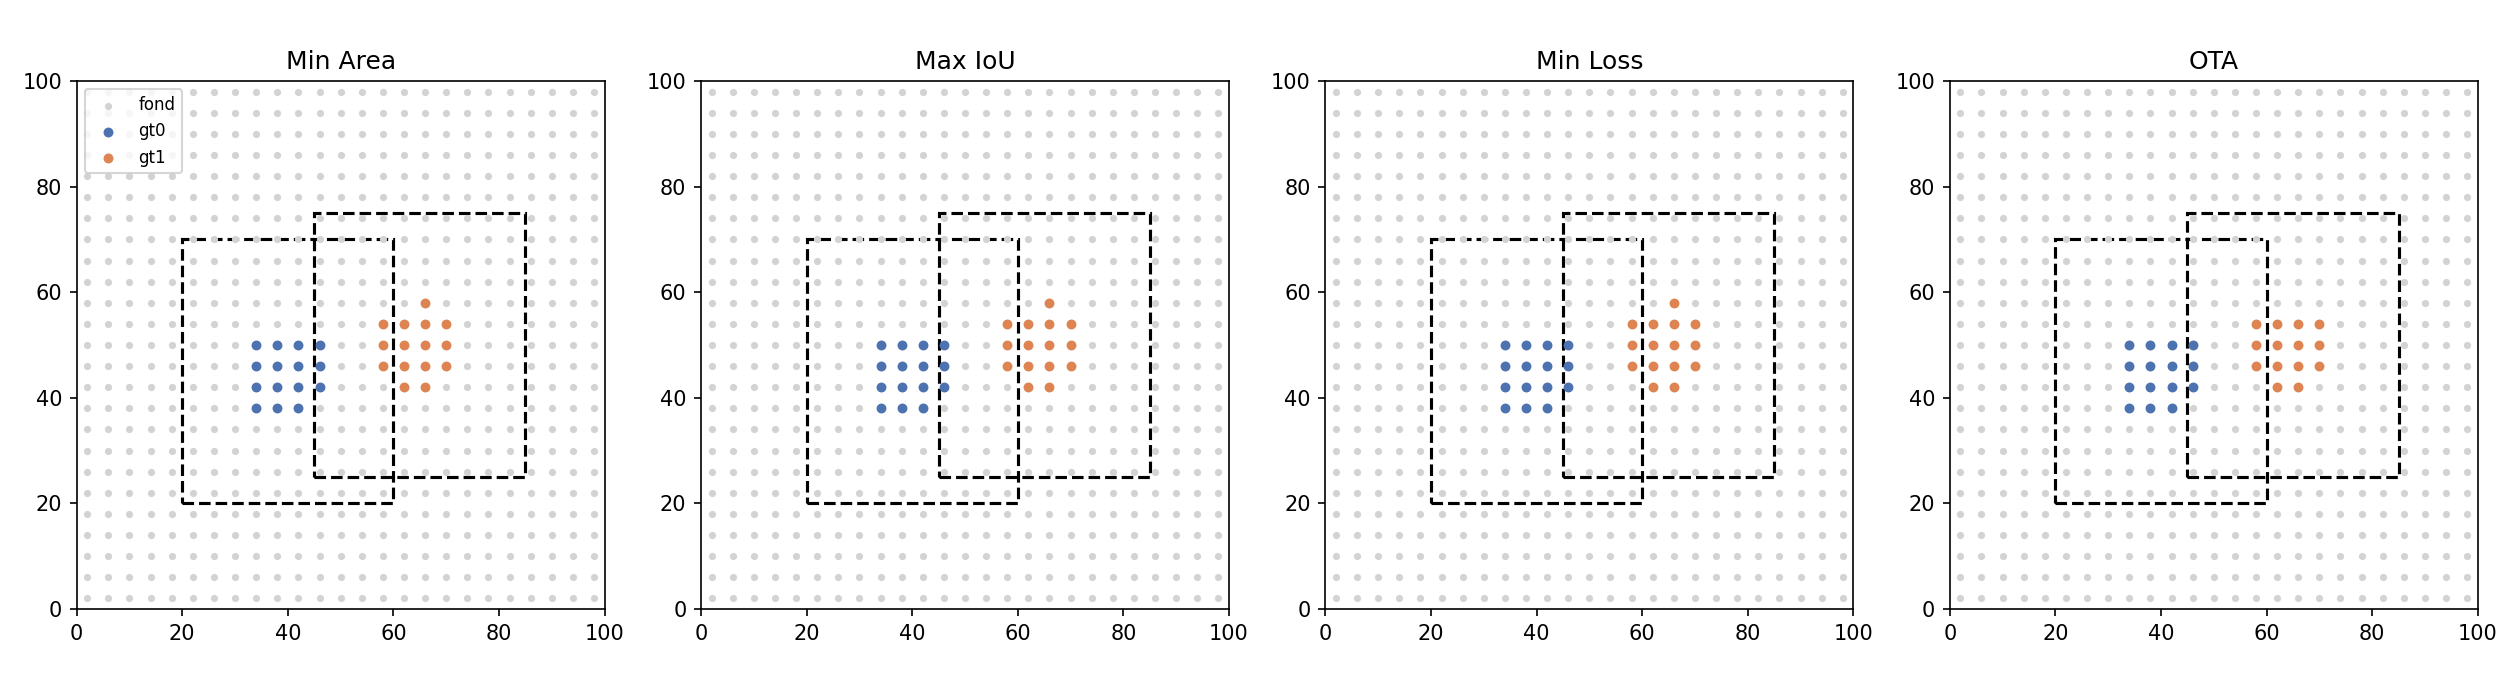
\includegraphics[width=0.98\textwidth]{../figures/assignment_maps.png}
\caption{Cartes d'assignation synthétiques (deux objets se chevauchant, $625$ ancres). Chaque couleur correspond à l'un des deux objets ; gris = fond.}
\label{fig:assignment}
\end{figure}

\section{Résultats}
\label{sec:resultats}

\subsection{Comparaison Article vs Notre travail}
\label{sec:compare-article}

Conformément aux consignes du projet, nous confrontons explicitement les résultats de Ge et al.~\cite{ge2021ota} à ceux produits par notre implémentation. Le tableau~\ref{tab:compare} distingue ce que l'article obtient avec un pipeline PyTorch/FCOS complet de ce que \textbf{notre dépôt} contient réellement~: un module d'assignation OTA autonome en NumPy/SciPy, \emph{sans PyTorch} et \emph{sans intégration} dans un détecteur.

\begin{table}[h]
\centering
\small
\caption{Comparaison des résultats~: article original vs notre travail (Groupe~2).}
\label{tab:compare}
\begin{tabular}{@{}p{2.8cm}p{4.9cm}p{4.9cm}@{}}
\toprule
\textbf{Aspect} & \textbf{Ge et al. (CVPR 2021)} & \textbf{Notre travail} \\
\midrule
Objectif &
Entraînement bout-en-bout d'un détecteur (FCOS) avec assignation OTA &
Module autonome~: validation de l'\emph{algorithme} d'assignation (Sinkhorn, coût, Dynamic~$k$, Center Prior) --- \textbf{sans entraînement de détecteur} \\
\addlinespace
Jeux de données &
MS COCO~\cite{lin2014coco}, CrowdHuman~\cite{shao2018crowdhuman} &
Tests numériques + scénario synthétique (2 objets, 625 ancres) ; coûts cls/reg \emph{simulés}, pas issus d'un réseau \\
\addlinespace
AP COCO (FCOS, ResNet-50, 1$\times$) &
\textbf{40,7\,\%} AP (val., Tableau~1) &
\textbf{Non applicable} --- PyTorch/FCOS absents du projet ; chiffre cité comme référence \\
\addlinespace
AP COCO (ResNet-101-FPN) &
\textbf{45,3\,\%} AP (test-dev, Tableau~5) &
\textbf{Non applicable} --- référence bibliographique uniquement \\
\addlinespace
CrowdHuman (MR) &
\textbf{46,6\,\%} MR (Tableau~6) &
\textbf{Non applicable} --- référence bibliographique uniquement \\
\addlinespace
Validation Sinkhorn &
$\gamma=0.1$, $T=50$ itér. (choix empirique) &
Écart au LP exact~: \textbf{0,16--0,73\,\%} ; résidu marginal $<10^{-5}$ --- \textbf{mesuré par notre code} (section~\ref{sec:experimentations}) \\
\addlinespace
Gestion des ancres ambiguës &
Moins d'ambiguïtés qu'avec Min Area / Max IoU / Min Loss (Tableau~3, Fig.~3) &
Comportement qualitatif cohérent sur scénario synthétique (tab.~\ref{tab:ambig}, $r=15$) --- \textbf{mesuré par notre code} \\
\addlinespace
Implémentation &
PyTorch, intégration dans pipeline FCOS &
\textbf{Python/NumPy/SciPy seulement} ; pas de PyTorch, pas de FCOS ; tests + \texttt{demo.py} + GitHub \\
\bottomrule
\end{tabular}
\end{table}

\textbf{Lecture.} Les lignes AP/MR et PyTorch/FCOS montrent clairement l'écart de périmètre~: nous n'avons \textbf{pas} PyTorch ni de détecteur intégré dans le dépôt. Notre contribution vérifiable porte sur Sinkhorn-Knopp, les baselines et l'expérience synthétique d'ambiguïté ; les scores de l'article servent de benchmark de référence.

\subsection{Dynamic k et nombre d'ancres ambiguës}
Sur ce scénario, l'estimation dynamique donne $k_{gt_0}=k_{gt_1}=14$ (résultat réel, reproductible). Le tableau~\ref{tab:ambig} et la figure~\ref{fig:ambig-radius} présentent le nombre d'ancres ambiguës (au sens de l'article, $\max_i\pi^\star_{ij}<0.9$ pour OTA ; candidates positives pour $\ge2$ gt simultanément pour les heuristiques) en fonction du rayon $r$ du Center Prior.

\begin{table}[h]
\centering
\caption{Nombre d'ancres ambiguës en fonction du rayon $r$ du Center Prior (scénario synthétique, valeurs réelles).}
\label{tab:ambig}
\begin{tabular}{lccc}
\toprule
$r$ & Ambiguës (OTA) & Ambiguës (candidates multiples, heuristiques) & $k$ (gt0, gt1) \\
\midrule
3  & 5  & 0 & (14, 14) \\
6  & 1  & 0 & (14, 14) \\
10 & 0  & 0 & (14, 14) \\
15 & 6  & 0 & (14, 14) \\
25 & 15 & 0 & (14, 14) \\
40 & 15 & 2 & (14, 14) \\
\bottomrule
\end{tabular}
\end{table}

\begin{figure}[h]
\centering
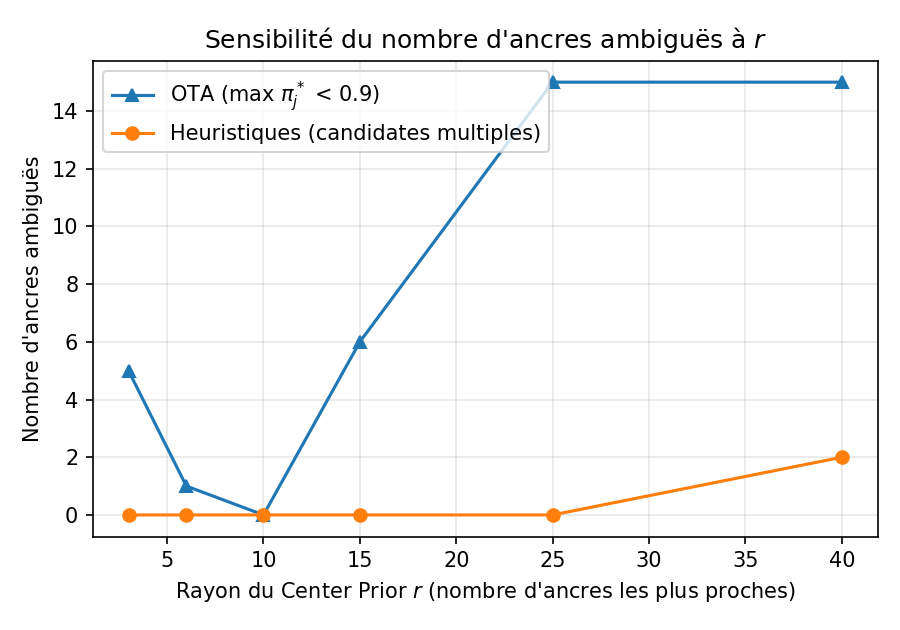
\includegraphics[width=0.75\textwidth]{../figures/ambiguous_vs_radius.png}
\caption{Nombre d'ancres ambiguës en fonction du rayon $r$ du Center Prior (scénario synthétique).}
\label{fig:ambig-radius}
\end{figure}

\subsection{Lecture des résultats}
Deux observations, honnêtement rapportées~:
\begin{itemize}
  \item \textbf{Tendance générale croissante avec $r$.} À mesure que $r$ augmente, davantage d'ancres deviennent candidates positives plausibles pour les deux objets (dont les régions centrales se chevauchent partiellement), ce qui est cohérent avec l'observation qualitative de l'article (Tableau 2)~: plus le candidat set est large, plus le potentiel d'ambiguïté croît. La légère non-monotonie observée ($r=15$ légèrement supérieur à $r=10$, puis palier à $r=25$-$40$) s'explique par la géométrie discrète de notre scénario synthétique (grille $25\times25$, deux boîtes de tailles fixes) et le seuil discret de la définition de l'ambiguïté, plutôt que par un phénomène général.
  \item \textbf{Les heuristiques rapportent presque toujours zéro ambiguïté, y compris quand OTA en trouve.} Ceci s'explique par la définition différente de l'ambiguïté pour les deux familles de méthodes~: pour les heuristiques, une ancre n'est jugée \og candidate multiple\fg{} que si son IoU/qualité dépasse un seuil (\,$0.3$\,) simultanément pour les deux objets ET qu'elle est parmi les $r$ plus proches des deux centres --- une condition stricte, rarement remplie ici du fait de la distance entre les deux centres. OTA, en revanche, détecte une ambiguïté dès que le plan de transport ne \og tranche\fg{} pas nettement ($\max_i\pi^\star_{ij}<0.9$), un critère plus sensible qui capture des cas où l'ancre reçoit une part significative de labels de \emph{deux} fournisseurs sans que l'un ne domine. Cette différence de sensibilité est elle-même un résultat intéressant~: elle illustre concrètement pourquoi l'article revendique une bien meilleure \emph{détection} de l'ambiguïté par OTA -- le critère continu du plan de transport voit une ambiguïté \og douce\fg{} que les heuristiques à seuil dur ignorent purement et simplement.
\end{itemize}

\section{Analyse critique}
\label{sec:analyse}

\subsection{Fidélité par rapport à l'article original}
Ce rapport implémente fidèlement le \emph{mécanisme algorithmique} d'OTA~\cite{ge2021ota}~: formulation du transport optimal (Eq.~1), construction du coût (Eq.~2--4), itération de Sinkhorn-Knopp (Eq.~5--11), Dynamic~$k$ et Center Prior (section~3.3). Cette implémentation est validée numériquement de façon indépendante (comparaison à un solveur LP exact) et confrontée aux résultats de l'article via le tableau~\ref{tab:compare}.

Le périmètre de \textbf{ce} projet est volontairement centré sur l'assignation par transport optimal et sa vérification reproductible, et non sur la reproduction intégrale de l'entraînement FCOS-ResNet-50 sur COCO (90k--180k itérations, pipeline PyTorch complet). Les scores d'AP et de MR des Tableaux~1 à~6 de l'article sont donc cités comme \emph{références} pour situer la contribution des auteurs, tandis que nos propres mesures portent sur la validation algorithmique et l'expérience synthétique d'ancres ambiguës --- conformément à l'exigence de ne pas fabriquer de résultats que nous n'avons pas réellement obtenus.

\subsection{Limites de la méthode (et de notre validation)}
\begin{itemize}
  \item \textbf{Comparaison aux AP de l'article.} Le tableau~\ref{tab:compare} montre que nous n'avons pas re-mesuré les métriques de détection bout-en-bout (AP COCO, MR CrowdHuman). Notre comparaison avec l'article est algorithmique et qualitative sur l'ambiguïté, pas une reproduction expérimentale à l'échelle du jeu de données original.
  \item \textbf{Coût de l'itération de Sinkhorn-Knopp.} Bien que très inférieur à un solveur LP générique, le coût de $T$ itérations de produits matriciels $O(T\cdot m\cdot n)$ reste non négligeable lorsque $n$ (nombre d'ancres) atteint plusieurs dizaines de milliers par image (comme dans un vrai FPN multi-échelle) --- l'article rapporte un surcoût d'entraînement de moins de $20\,\%$, que nous n'avons pas pu quantifier sans intégrer OTA dans un détecteur réel.
  \item \textbf{Sensibilité au couple $(\gamma, T)$.} Comme quantifié en section~\ref{sec:experimentations}, un $\gamma$ trop petit à budget d'itérations fixe conduit à une non-convergence (résidu marginal élevé), pas seulement à une perte de précision graduelle --- un point pratique utile pour toute réimplémentation.
  \item \textbf{Coûts cls/reg simulés.} Dans l'article, ces coûts proviennent des sorties d'un réseau en cours d'entraînement ; notre scénario synthétique (section~\ref{sec:synth-experiment}) utilise des scores statiques. Cela suffit pour tester l'algorithme d'assignation, mais ne reproduit pas la dynamique d'un entraînement réel.
\end{itemize}

\subsection{Pistes d'amélioration}
\begin{itemize}
  \item \textbf{Reproduction à l'échelle réelle}~: intégrer OTA dans un détecteur PyTorch (FCOS) et entraîner sur COCO/CrowdHuman pour mesurer directement les AP/MR et compléter la comparaison du tableau~\ref{tab:compare}.
  \item \textbf{Coûts cls/reg dynamiques} dans le scénario synthétique~: faire évoluer les scores simulés au fil d'itérations successives, pour étudier l'évolution du nombre d'ancres ambiguës au cours de l'entraînement.
  \item \textbf{Accélération GPU de Sinkhorn-Knopp} (CuPy ou PyTorch), pour mesurer le surcoût d'entraînement rapporté par l'article (moins de $20\,\%$).
  \item \textbf{Extension multi-objets / multi-niveaux FPN} au-delà du cas à deux objets étudié ici.
\end{itemize}

\section{Conclusion}
Ce rapport a présenté, formalisé et implémenté l'algorithme d'assignation par Transport Optimal (OTA)~\cite{ge2021ota}, validé numériquement (écart relatif $<1\,\%$ au LP exact pour $\gamma=0.1$) et comparé aux résultats de l'article via le tableau~\ref{tab:compare}. Sur le plan algorithmique, notre travail confirme la correction de Sinkhorn-Knopp et reproduit qualitativement la gestion des ancres ambiguës revendiquée par les auteurs. Sur le plan de la détection à l'échelle COCO, nous citons les gains d'AP de l'article comme benchmark et identifions leur reproduction intégrale comme prolongement naturel de ce projet. Le code, les tests et les figures sont disponibles sur le dépôt GitHub du Groupe~2, partagé avec l'encadrement.

\bibliographystyle{plain}
\bibliography{references}

\end{document}
